\documentclass{oci}
\usepackage[utf8]{inputenc}
\usepackage{lipsum}

\title{Bus de turismo}

\begin{document}
\begin{problemDescription}
  La empresa de turismo \emph{Al Sur del Mundo} tiene una flota de buses que
  utiliza para transportar a sus pasajeros en cada uno de los recorridos que
  ofrece a lo largo del país. 
  Todos los buses en la flota tienen 48 asientos distribuidos tal como se
  muestra en la siguiente figura.

  \begin{center}
  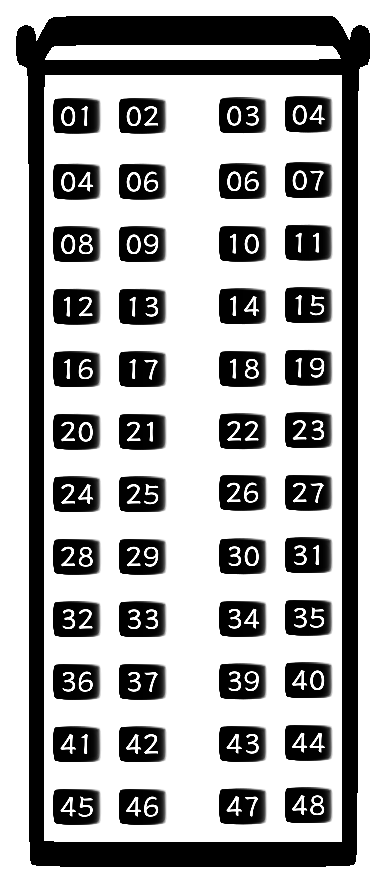
\includegraphics[angle=270,origin=c,scale=0.8]{bus.eps}
  \end{center}
  \vspace{-9em}
  A menudo la gente hace reservas para grupos de más de una persona.
  Como es de esperar, a las personas les gusta siempre sentarse junto a alguien
  de su mismo grupo.
  Se considera que dos personas están juntas si están sentadas en la misma fila
  y no están separadas por el pasillo.
  A una persona que viaja sola nunca le importará donde sentarse.

  Durante el último tiempo han surgido algunas inquietudes dentro del directorio
  pues creen que mucha gente está quedando separada de su grupo lo que
  estaría provocando mucha incomodidad entre los clientes.
  Los guías que trabajan directamente dentro de los buses creen que esto no es
  cierto pues ellos ayudan a los pasajeros a sentarse de forma óptima de modo
  que la máxima cantidad de pasajeros quede junto a alguien de su grupo.

  ?`Podrías ayudar a los ejecutivos a determinar si la situación es realmente un
  problema?
  Dado el número de gente en cada grupo, y suponiendo que todos se sientan de
  forma óptima, tu tarea es determinar la cantidad de gente no queda sentada
  junto a alguien de su grupo.
  
\end{problemDescription}

\begin{inputDescription}
  La primera línea de la entrada contiene un entero $N$ correspondiente a la
  cantidad de grupos que han hecho reserva.
  Cada una de las siguiente $N$ líneas contiene un entero $A_i$ ($A_i > 0$)
  correspondiente a la cantidad de gente en cada uno de los grupos.
  La cantidad total de gente nunca será mayor que 48.
\end{inputDescription}

\begin{outputDescription}
  La salida debe corresponder a un único entero correspondiente a la cantidad de
  gente que no queda sentada junto a alguien de su grupo.
\end{outputDescription}

\section*{Subtareas y puntaje}
Este problema no contiene subtareas. Se probarán varios casos de prueba y se
otorgará puntaje puntaje de acuerdo a la cantidad de casos de prueba correctos.

\begin{sampleDescription}
\sampleIO{sample-1}
\sampleIO{sample-2}
\end{sampleDescription}

\end{document}